\section{实验}

我们报告三件东西：一个可执行工件、一次带预注册假设的确定性零模型消融，
以及一次说明性的真实宿主试点。

\subsection{工件与可复现性}

引擎是零依赖 Python、不调用任何模型；插件是 JavaScript 重实现。
可行性由断言保证：14 个测试文件中的 892 条 Python 断言，以及 396 条插件断言
（188/148/45/15）；后一个数字取自 2026-10-27 的审计快照，且没有为本文重新执行。
为第~\ref{sec:method} 节在此重新执行的是：161、65 与 26 条断言，全部通过。
提交时三项漂移检查均为绿：一份 66 键的规则/引擎/插件比对、一份契约摘要，
以及一次实现状态矩阵检查。确定性是被强制的：固定时钟（每轮 60\,s）、不使用墙钟、
无随机、无网络。相同配置、存储与脚本给出逐字节相同的运行结果；
本次运行报告 \texttt{model\_calls=0}、\texttt{network\_calls=0}、两个写出文件，
以及 51/51 项校验通过。

\subsection{确定性三臂消融}

\paragraph{协议。} 一个 100 轮脚本由混沌与回放语料确定性生成
（SHA-256 \texttt{701ff06a0b37\ldots}）：21,610 个字符，对 24,000 字符的窗口，
最大用量比 $0.9004$，相变监控在第 73--100 轮触发（28 轮）。
十二个探针覆盖长程设定（A）、被取代的值（B）、干扰过载的设定（C），
以及一个构造出的「高频但陈旧」偏好（D，30 次访问，最后一次在 100 天前）；
两个未命中探针位于第 86--87 轮。命中由条目敏感性判定。
\textsc{Baseline}（基线）注入最近三轮原始对话，没有记忆或控制层；
\textsc{Basic}（基础）使用预算化、以查询为条件的召回，关闭 ACT-R 通道
（\texttt{actrWeight=0}）、使用静态权重、没有控制层；
\textsc{Full}（完整）使用默认设置，即双通道 potency、动态权重与全部四个控制子系统。
在线上兼容的核心上，测试装置与流水线在 100/100 轮上一致；标签开启时的分歧记录在结果文件中。
表~\ref{tab:ablation} 与图~\ref{fig:retention} 报告结果。

\begin{table*}[t]
\centering\footnotesize
\caption{三臂消融。SFR：按类别与总体的设定遗忘率（setting-forgetting rate）；
NHD：未命中纪律（括号内为字面变体）；IIR：对抗干扰比；telemetry：相变/锚点轮数、
fallback 标记数（实际丢弃）、UCA-08 记录数。来源：
\texttt{results/abl-20261027-003626-engine.json}，字段
\texttt{conditions.<arm>.metrics.*} 与 \texttt{conditions.<arm>.telemetry.*}；
校验器 51/51。}
\begin{tabular}{@{}l cccc c c c c c ccc c@{}}
\toprule
 & \multicolumn{4}{c}{按探针类别的 SFR} & & & & & & \multicolumn{3}{c}{越狱（\%）} & \multicolumn{1}{c}{遥测}\\
\cmidrule(lr){2-5}\cmidrule(lr){11-13}\cmidrule(lr){14-14}
臂 & A & B & C & D & SFR$_{\text{text}}$ [95\% CI] & SFR$_{\text{id}}$ & IIR & NHD & UCE & in & fp & script & ph/anc/fb/08 \\
\midrule
Baseline & 1.00 & 1.00 & 1.00 & 1.00 & 1.00$^{\ddagger}$ & $\varnothing$ & $\varnothing$ & $\varnothing$ & $0^{\dagger}$ & $\varnothing$ & $\varnothing$ & $\varnothing$ & 0/0/0/0 \\
Basic & 0.00 & 0.00 & 0.00 & 1.00 & 0.25 [0.05, 0.57] & 0.25 & 0.56 & 1.00 (0.00) & $0^{\dagger}$ & $\varnothing$ & $\varnothing$ & $\varnothing$ & 0/0/0/0 \\
Full & 0.00 & 0.00 & 0.00 & 0.00 & 0.00 [0.00, 0.26] & 0.00 & 0.47 & 1.00 (0.00) & $0^{\dagger}$ & 1.00 (25) & 0.00 (294) & 0.00 (6) & 28/28/4(0)/62 \\
\bottomrule
\end{tabular}

\vspace{2pt}
\raggedright\scriptsize
$\varnothing$：不适用；该单元格是带原因的 \texttt{null}，从不是零。
$^{\ddagger}$：按构造——一个三轮窗口不可能包含一枚在第 85 轮之前埋下的设定。
$^{\dagger}$：结构性的零，因为所有注入条目都是 active 且由用户显式给出。
\end{table*}

\paragraph{结果。} 两个 LINGSHU 臂都完美召回了九个 A/B/C 探针，
而基线的 $1.00$ 是窗口算术——按构造就是定义性的——因此我们不把基线—系统的差异当作效应量。
两臂只在 D 类上分离：\textsc{Basic} 三个全丢，\textsc{Full} 三个全召回，
于是 $0.25$ 对 $0.00$（$p=0.125$，三对不一致，不显著）。
在十二个配对探针下，精确符号检验在 $\alpha=0.05$ 时只能检出
$5/12\approx0.42$ 的差异（Bonferroni 校正后为 $6/12=0.50$），
而一个只有三项的类别根本无法达到显著；因此我们只报告方向与逐探针细节。
顺序置换不改变 SFR，但会移动锚点计数（28/62/21）：保持率对顺序稳健，相变时序则不是。

预注册结果连同失败一并报告。P1b 在其点估计上通过，但未通过置信准则
（Basic 的 Clopper--Pearson 上界为 $0.572$，而要求为 $0.45$）。
P2 在忠实于代码的谓词下通过，而字面子串谓词因为引擎措辞不同返回 $0.00$；两个数字都成立。
P3 不可评估，因为两臂都是结构性的零。P5 不可判定：
分布内越狱被阻断 25/25，误报为 0/294，脚本化用户轮次越狱为 0/6，
但留出集从未被撰写，因此该单元格为 \texttt{null}。
P6 通过（\textsc{Full}：28 个相变轮、28 个锚点、4 个 fallback 标记、62 条 UCA-08 记录；
\textsc{Basic} 全为零）。P7 在单锚点开销上通过（$+100$ 到 $+124$ 字符），
但未通过其字面意义上的两倍阈值。

\paragraph{如何读相变窗口。} 两个阈值都落在本次运行内：用量比在第 73 轮越过 $0.70$（相位 \emph{shift}）、在第 85 轮越过 $0.85$（相位 \emph{critical}），因此 shift 窗口是第 73--100 轮，critical 窗口是第 85--100 轮（见第~\ref{sec:method:phase} 节）。遥测显示阈值在实践上改变了什么，而不只是公式：\textsc{Full} 记录 28 个相位轮、28 个锚点、4 个 fallback 标记与 62 条 UCA-08 记录，\textsc{Basic} 则是 0/0/0/0；图~\ref{fig:retention} 轴下方的锚点条带从第 73 轮开始，并贯穿 critical 窗口。该图也说明相变监控本身为何不能提升保持率：\textsc{Basic} 与 \textsc{Full} 的注入集合完全相同，因此阴影带标记的是控制面开始支付 prompt 预算成本的时刻，而不是记忆改善的时刻。因此我们把 70\%/85\% 阈值读作锚定与审计的升级点，而不是学习或检索收益。

\subsection{真实宿主试点}

十个单元格跑在一个宿主、一条模型路由上，每格一次运行；细节见附录~\ref{app:hostpilotdata}。方法学发现是：把 100 轮对话压成一条 78\,KB 的请求会把查询稀释到“以查询为条件的召回不再命中”（\textsc{Full} 报告 \texttt{matched=0}），并且控制层在所有单元格中都没有触发（闸门全程返回 \texttt{allow}、UCA 列表为空）。这是在 $n=1$ 上的机制演示，不是幻觉率。

\begin{figure*}[t]
\centering
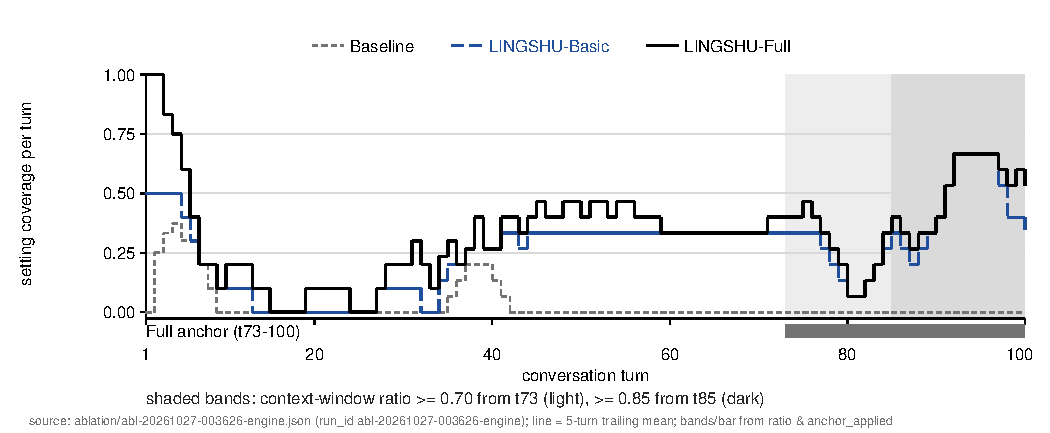
\includegraphics[width=\textwidth]{figures/fig2-retention.pdf}
\caption{100 轮脚本中每轮的设定覆盖率：
$y_t = |\mathcal{S}^{\mathrm{inj}}_t \cap \mathcal{S}^{\mathrm{act}}_t| /
|\mathcal{S}^{\mathrm{act}}_t|$，即当前活跃的被埋设定出现在注入上下文中的比例
（画成 5 轮尾部均值；原始逐轮均值对 \textsc{Baseline}、\textsc{Basic}、\textsc{Full}
分别为 0.025、0.260 与 0.327）。\textsc{Basic} 与 \textsc{Full} 按设计重叠：
控制面不改变召回成员集合。阴影带标出相变窗口（第 73 轮起 $r \ge 0.70$，
第 85 轮起 $r \ge 0.85$）；坐标轴下方的条带标出 \textsc{Full} 注入首尾人格锚点的轮次。
来源：\texttt{abl-20261027-003626-engine.json} 中的
\texttt{conditions.<arm>.turns[].\{setting\_ids\_injected, active\_setting\_ids,
ratio, anchor\_applied\}}。}
\end{figure*}

\subsection{混沌注入下的鲁棒性}

\paragraph{协议。} 从系统\emph{外部}注入三种故障；\texttt{plugin/}、\texttt{engine/} 与 \texttt{rules/} 在战役前后做了哈希，未发生变化。每个用例运行在各自的 \texttt{DSH\_HOME} 中，其 profile 副本通过目录联接（directory junction）链接到仓库插件，因此被测代码就是当前参考实现，注入被限制在宿主层与磁盘上的记忆状态内。所有运行都是固定短 prompt 的 headless CLI 调用；转录、插件状态、审计日志与最终 prompt 都写入磁盘并离线分析。每个注入点只运行一次（$n=1$）；本节不进行任何红队变异。

\emph{A，传输故障。} 宿主的模型端点通过文档化的 \texttt{DEEPSEEK\_BASE\_URL} 环境变量被重定向到本地 mock，该 mock 返回 HTTP 500、合法但空的 200 响应、携带伪造答案的合法 200 响应，或接受连接但永不回答。

\emph{B，记忆故障。} 记忆库在文件层被破坏，但不触碰 \texttt{memorywriter.js}：(B1) \texttt{memory.jsonl} 被替换为目录，因此读取以 \texttt{EISDIR} 失败并被吞掉，而写会抛错；(B2) 一个可读但脏的库被填入一条撕裂的 JSON 行、一个重复 id（后一行是取代墓碑），以及两行共享 $(\textsc{subject},\textsc{relation})$ 但 \textsc{object} 不一致的 active 条目。预热状态模板被预先写入，以免冷启动门控掩盖效果；该设置是合成的，并已如实披露。

\emph{C，上下文灌水。} 一条确定性的 150{,}000 字符垃圾流（按插件 3 字符/token 估算器约 50k token）作为用户消息传入，同时 \texttt{LINGSHU\_CONTEXT\_WINDOW} 把插件感知窗口固定为四个值；一个 mock 端点记录拼装出的请求体，因此本次运行不消耗模型 token。

\begin{table*}[t]
\centering\footnotesize
\caption{故障注入矩阵。每个单元格都是一次运行中的观测值；$\varnothing$ 标记被注入故障变得不适用的量，而绝不是零。A：同一固定 prompt 上的五种传输模式。B：在合成预热状态上的三次 headless 运行。C：同一 150k 字符输入上的四个窗口值，外加精确的边界括测。来源：\texttt{experiments/chaos-injection/out/}。}
\begin{tabular}{@{}l l l l@{}}
\toprule
故障 & 注入模式 & 控制面观测 & 关键数字 \\
\midrule
A 传输 & HTTP 500 & 错误由宿主暴露；注入仍运行了一次 & 7 次尝试，17.99 s，退出码 1 \\
        & 空 200 & 空最终消息被透传，退出码 0 & 最终长度 0 \\
        & 伪造 200 & 伪造文本到达 stdout，退出码 0 & 最终长度 23 \\
        & 永不回答 & 150 s 窗口内无客户端超时 & $\ge$150.03 s \\
        & 全部模式 & \texttt{blocked=false}；宪法在 prompt 中 & 5/5 \\
B 记忆 & 库为目录（B1） & \texttt{hook\_error}=1（\texttt{EISDIR}）；写入 0；回复返回 & 9.851 s，退出码 0 \\
        & 脏库（B2） & \texttt{fallback=true}，\texttt{drop style}；被取代值未被召回 & 21.046 s，退出码 0 \\
        & 干净对照（B0） & 风格与组织段被注入；无 fallback & 45.654 s，退出码 0 \\
C 上下文 & 4 个窗口，150k 字符 & \texttt{normal/shift/shift/critical}；宪法 4/4 & 比率 0.681/0.701/0.721/0.851 \\
        & 边界括测 & \texttt{0.7000}$\to$normal，\texttt{0.7006}$\to$shift；\texttt{0.8500}$\to$shift，\texttt{0.8507}$\to$critical & 8 次 headless 调用，0 次模型调用 \\
\bottomrule
\end{tabular}
\end{table*}

\paragraph{传输故障（A）。} 一个普通 200 响应在 2.84\,s 内完成。HTTP 500 被宿主以指数退避重试七次（尝试间隔 0.55、0.96、1.92、4.25、7.51\,s），并在 17.99\,s 后暴露一行错误（\texttt{dsh: SERVER: mock upstream 500}），以非零码退出，且\emph{没有}伪造文本。一个永不回答的端点在 150\,s 观测窗口内没有响应，并被 harness 终止，而不是被客户端超时终止。在全部五种模式中，插件恰好执行了一次 pre-step 注入，宪法段始终留在最终 prompt 中，\texttt{state.control.blocked} 保持 false，且没有记录 hook 错误。空的 200 响应被作为空最终消息透传（退出码 0），伪造的 200 响应逐字到达 stdout（23 个字符）。因此控制面从不把传输失败转化为伪造内容，但它既不增加传输超时，也不增加输出校验器：这些仍是宿主层的职责。

\paragraph{记忆故障（B）。} 在干净库（B0）下，注入的 prompt 携带宪法、元认知、组织与风格段，且没有 fallback 标记。把库替换为目录（B1）会引发一次 \texttt{hook\_error}（\texttt{Error: EISDIR ... write}），\texttt{stateWrites} 停在运行前的值，但该轮仍以退出码 0 结束并返回 364 字符的回答，宪法与风格段完好——功能 fail-open，记忆被隔离。我们报告两条告诫而不是抹平它们：回复断言事实已被记录，尽管写入可证明地失败了；模型自己的状态叙述引用了合成的预热模板计数器，因此判断只使用磁盘证据。在脏库（B2）下，召回返回 \texttt{mem\_002} 与 \texttt{mem\_003}，而被取代的墓碑 \texttt{mem\_001} 缺席；$(\textsc{subject},\textsc{relation})$ 对上的冲突被归类为未解决，多样性守卫设置 \texttt{fallback=true} 与 \texttt{dropDomains=["style"]}，最终 prompt 失去风格段但保留冲突澄清标记与宪法块，\texttt{verdict} 仍为 \texttt{allow}、\texttt{blocked} 为 false，模型请用户澄清而不是选择某个值。脏库还暴露了一个规则桩工件：\emph{问题}“我的项目代号是什么？”被抽取为一条 object 为疑问词“什么”的事实，且在 B2 中它的写入取代了这两行冲突记录（\texttt{supersedeEvents}=2）。该工件不能被读作收益：它意味着下一轮的冲突可能被查询本身抹掉。\footnote{逐字节的中文 prompt 标记与冲突键逐字记录在 \texttt{experiments/chaos-injection/out/} 中；本文用 ASCII 呈现它们，以便源码用标准 T1 字体编译。}

\paragraph{上下文灌水（C）。} 四个窗口的实测用量比（保留四位小数）为 0.6806、0.7006、0.7206 与 0.8507；相位分别为 \texttt{normal}、\texttt{shift}、\texttt{shift}、\texttt{critical}。两个精确边界括测钉住阈值：在 $\ge$ 语义下，最大的 shift 窗口是 71{,}490（$r=0.700000$），而 71{,}491 为 \texttt{normal}；最大的 critical 窗口是 58{,}874（$r=0.8500017$），而 58{,}875 为 \texttt{shift}。四位小数显示是个陷阱：窗口 71{,}493 打印 \texttt{0.7000} 却仍是 \texttt{normal}，58{,}876 打印 \texttt{0.8500} 却仍是 \texttt{shift}；只有未舍入的比率是决定性的。插件对名义 50{,}000 token 的估计是 50{,}043：其输入是 150{,}127 字符的 JSON 消息信封（\texttt{role}/\texttt{content} 包装的 127 个字符），因此所有实测比率都比名义值高约 0.0006。宿主随后渲染 151{,}936 个 JSON 字符（50{,}646 token），在用户消息后追加一个 1{,}809 字符的指令块；因此插件把模型可见输入低估了约 $1.2\%$。物理占用约为模型 1M token 窗口的 $5.2\%$：这里的窗口是实验室覆写，比率是相对控制信号，而不是饱和测量。

没有发生截断：4/4 次运行中完整输入都出现在 mock 请求体里（\texttt{prompt\_full\_in\_body}），截断率为 0.0，宪法段在 4/4 次请求中都存在。但锚点投递暴露了一个真实的“一次拼装滞后”。插件自己的 prompt 预览在设置 \texttt{prefeed} 时携带 head 锚点，在 \texttt{critical} 时携带 head 与 tail 两个锚点；而到达模型的\emph{请求}在 8/8 次观测中携带的是\emph{上一轮}的锚点集合。最清楚的例子是第一个 \texttt{critical} 轮：其预览有 head 与 tail，其请求只有 head，只有下一次请求才两个都有。机制在宿主侧：agent loop 在发出 \texttt{agent/pre-step} 之前就拼装好 system prompt，而插件在该钩子中更新相位状态（在 \texttt{dsh-agent-loop} 中拼装先于钩子四行源码）；插件无法改写已经拼好的请求。即使被投递，tail 锚点也止于 2{,}906 个字符中的 system 偏移 229，即模型可见文本的约 $0.17\%$，因此“head 与 tail”指的是插件七段式 prompt 的第 90/140 段，而不是请求的绝对首尾。因此单轮或单次部署不应期望 critical 锚点在产生 critical 比率的那一轮就生效。

\begin{figure*}[t]
\centering
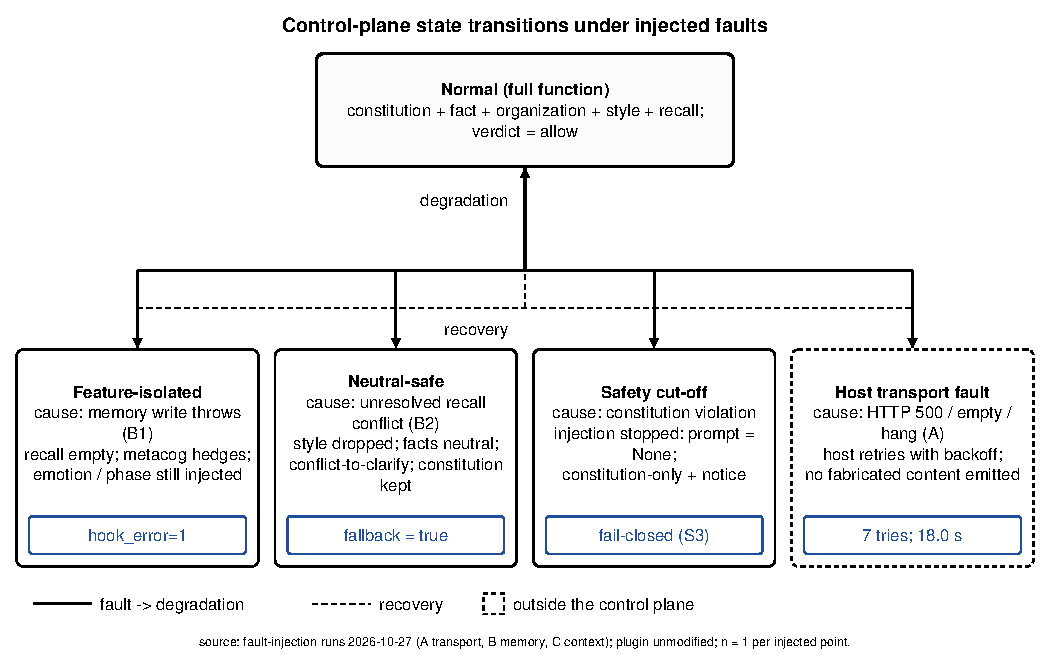
\includegraphics[width=0.98\textwidth]{figures/fig3-robustness.pdf}
\caption{注入故障下控制面的状态转移。正常运行沿三条不同路径降级——记忆写失败下的功能隔离（B1）、未解决召回冲突下的中性安全输出（B2）、宪法违规下的安全切断（\texttt{docs/22} 中已有的 STPA 证据）——而传输故障仍在控制面之外（A）。实线弧是故障到降级的转移，虚线弧是恢复。逐点证据与精确数字在 \texttt{experiments/chaos-injection/out/}；每个注入点 $n=1$，插件未改动。}
\end{figure*}

\paragraph{这种不对称保证了什么。} 在三个场景中，控制面的不对称恰好朝一个方向：当涉及\emph{安全}谓词时，闸门 fail-closed，停止注入而不是软化拒绝；当涉及\emph{功能}时，失败是 fail-open——记忆隔离与中性安全输出让该轮保持可用，宪法块被保留，且没有故障被静默转化为内容——因此 \emph{LINGSHU 的非对称降级机制（安全 fail-closed、功能 fail-open）在极端混沌下保证系统可用性}。这句话的范围是控制面。传输故障被暴露，但插件既不超时也不重试；模型输出不被插件校验；且一条 B1 回复断言了一次并未发生的持久化；因此传输故障下的可用性取决于宿主，输出真实性仍在机制职责之外。

\subsection{证据的范围}

这些实验确立的是契约行为与机制可达性，而不是模型层面的效应量：引擎不调用模型，宿主运行是每个单元格一次、单一模型路由，混沌故障是 $n=1$ 的合成注入，而不是生产故障的样本。有两项结构性限制值得在此点名，因为它们界定了主张的形状：到达模型的锚点集合比插件相位慢一次拼装，因此第一个 critical 请求只携带 head 锚点；宿主运行涉及真实模型，因而并非确定性，这正是上述每条主张都绑定到证据文件中的字段、而不是一句总结的原因。参数、样本与环境限制的完整清单统一收口在第~\ref{sec:limitations} 节。
